\documentclass[12pt, a4paper]{article}
\usepackage[utf8]{inputenc}
\usepackage[hmargin=2.5cm, vmargin=3.2cm]{geometry}
\usepackage{enumitem}
\usepackage{graphicx}

\title{
Master MVA -- Biostatistiques
}
\author{
Antoine Moulin \\
Telecom Paris \& ENS Paris-Saclay \\
\tt antoine.moulin@telecom-paris.fr
}
\date{31 Mars 2020}

\setlength{\parindent}{0pt}
\setlength{\parskip}{1em}


\begin{document}

\maketitle

\section{Premier problème}

Cette question porte sur l’article \cite{hernan18} par Miguel Hernàn.

\begin{enumerate}
    \item \textbf{Décrivez la problématique soulevée par l’auteur et qui justifie cet article ? En quoi l’approche classique de l’analyse de telles données peut conduire à des biais ?}
\end{enumerate}

    L'objet de cet article est d'utiliser des données d'observation afin d'estimer de façon non biaisée l'effet de la durée d'un traitement sur le taux de survie.
    
    A la différence des essais randomisés qui regroupent les patients en fonction de la durée de traitement qui leur est assignée, un usage naïf des données -- qui ne contiennent que la durée de traitement réalisée et non la durée assignée -- conduirait à une comparaison biaisée entre les patients non traités, ceux traités à court terme et ceux traités à long terme. En effet, les patients traités longtemps sont ceux qui, par définition, ont survécu longtemps. C'est un biais connu appelé le biais d'immortalité. Par exemple, si l'on souhaite calculer la probabilité de mourir pour un groupe non traité et un groupe traité pendant deux ans, le calcul pour le second groupe se fera sur le sous-groupe de patients ayant survécu durant toute la durée du traitement, en excluant les patients morts en cours de traitement (par exemple au bout d'un an).
    
    Si des méthodes existent pour régler ce problème, certaines ne permettent pas d'estimer le risque absolu ou de faire des ajustements en présence de facteurs de confusion. La méthode présentée dans cet article n'a pas ces limitations.

\pagebreak
\begin{enumerate}[resume]
    \item \textbf{Décrivez la proposition de l’auteur pour contourner cette difficulté.}
\end{enumerate}

    L'auteur propose une méthode articulée en trois étapes : clonage, censure et pondération.
    
    \textbf{Clonage}. On rappelle que dans les données d'observation, la variable donnant la durée de traitement assignée n'est pas disponible. Pour surmonter ce problème, l'auteur propose de la créer. Pour ce faire, on assigne à chaque patient toutes les stratégies de traitement compatibles avec les données disponibles à l'instant initial, créant ainsi des clones. Si le patient X n'a pas reçu de traitement à l'instant initial, la durée de traitement est nulle. Si au contraire il a reçu un traitement à l'instant initial, alors on lui assigne toutes les durées de traitement possibles. Cela revient à créer autant de clones qu'il n'y a de durées de traitement, chaque clone ayant une durée de traitement différente. Par exemple, si la durée peut être de un ou deux ans, deux clones X.a et X.b seront crées, l'un étant traité un an et l'autre deux.
    
    \textbf{Censure}. La deuxième étape consiste à censurer les patients ne respectant pas la stratégie qui leur est assignée. Par exemple, si un patient qui devait être traité un an continue de prendre le traitement au bout d'un an, il est censuré.
    
    Bien que ceci permette d'éviter le problème du  biais d'immortalité, se restreindre aux patients non censurés n'est pas suffisant car cela induit un biais de sélection, que la troisième étape permet de régler.
    
    \textbf{Pondération}. Cette étape consiste à affecter à chacun des patients une pondération. Les patients censurés reçoivent un poids nul, tandis que les patients non censurés reçoivent un poids égal à l'inverse de la probabilité de ne pas être censuré, le but étant de simuler une population dans laquelle personne n'est censuré car tout le monde a suivi la stratégie assignée.


\begin{enumerate}[resume]    
    \item \textbf{Quelle autre approche de modélisation pourrait être utilisée pour analyser correctement ce type de données ?}
\end{enumerate}

    Une alternative à la méthode précédente en trois étapes permettant de régler le problème du biais d'immortalité, d'estimer le risque absolu et de gérer les facteurs de confusion serait d'utiliser la formule g de Robins JM. Néanmoins cette méthode est plus complexe à utiliser que la méthode décrite ici, elle requiert des compétences en programmation et nécessite d'entraîner plusieurs modèles.

\pagebreak
\section{Deuxième problème}

Vous avez ci-joint l’article \cite{chinazzi19} par Chinazzi et coll. (article et matériel supplémentaire).

\begin{enumerate}
\item \textbf{Décrivez l’approche de modélisation utilisée.}
\end{enumerate}

Afin de modéliser la propagation de l'épidémie COVID-19 dans le monde, les auteurs utilisent le modèle GLEAM (\textit{Global Epidemic and Mobility Model}), qui est un modèle individuel, stochastique et spatial. Cela signifie qu'il représente la population mondiale comme un réseau de sous-populations situées près de pôles de transports, comme un aéroport, ces derniers permettant de connecter les différents groupes d'individus. Ce réseau est construit à partir de données réelles et la diffusion de l'épidémie se fait au niveau individuel. La transmission d'un individu à l'autre est modélisée par des processus stochastiques, et chaque individu est dans l'un des états suivants :
\begin{itemize}
    \item[-] S (\textit{Susceptible}). Ce sont les individus pouvant être contaminés par des personnes infectées (dans l'état I ci-dessous), passant ainsi dans l'état L.
    \item[-] L (\textit{Latent}). Il s'agit d'un état intermédiaire entre S et I, i.e. un individu a été contaminé mais n'est pas encore contagieux. On suppose que cette période a la même durée que la période d'incubation.
    \item[-] I (\textit{Infectious}). Un individu dans un état latent devient contagieux, passant ainsi dans l'état I.
    \item[-] R (\textit{Removed}). Lorsque l'individu n'est plus contagieux, i.e. lorsqu'il est guéri, isolé, hospitalisé ou mort, il passe dans l'état R et n'est plus un danger pour les autres individus.
\end{itemize}

Une fois ce modèle défini, il est possible de fixer les paramètres concernant la période d'incubation (durée de l'état L) et la période de contagion (durée de l'état I), permettant de calculer le temps de génération (moyenne des deux temps précédents) et de générer plusieurs scénarios possibles.

\begin{enumerate}[resume]
\item \textbf{Comment le modèle est-il calibré ?}
\end{enumerate}

Dans l'hypothèse où l'épidémie a débuté entre mi-novembre et début décembre à partir de 40 cas d'origine zoonotique, le but est de calculer, pour chaque temps de génération $T_g$, la distribution \textit{a posteriori} du coefficient de reproduction $R_0$.

Pour ce faire, on simule des épidémies à partir d'un coefficient de reproduction tiré aléatoirement et de façon uniforme entre 1.5 et 4. Il est ensuite possible de calculer la distribution du taux de croissance des cas de COVID-19 importés vers des sites internationaux pendant la croissance exponentielle de l'épidémie, dénotée $P(D)$, ainsi que la vraisemblance $P(D|R_0)$. La formule de Bayes permet d'en déduire la distribution \textit{a posteriori} $P(R_0|D)$.

On sélectionne ensuite les simulations qui sont en accord avec les données observées jusqu'au 23 Janvier 2020.

\begin{enumerate}[resume]
\item \textbf{Décrivez les résultats obtenus.}
\end{enumerate}

Le résultat le plus important à retenir de cette étude est qu'une restriction des déplacements ne sera réellement efficace que si elle est couplée à une réduction du taux de transmission d'au moins 50\%. En effet, comme on peut le voir figure \ref{fig:results-effect-travel-ban}, dans le cas où le taux de transmission n'est pas réduit, l'interdiction des voyages ne fait que retarder l'épidémie de quelques jours, mais sans l'atténuer (voir figures 1A et première partie de 1D). \\

\begin{figure}[!h]
    \centering
    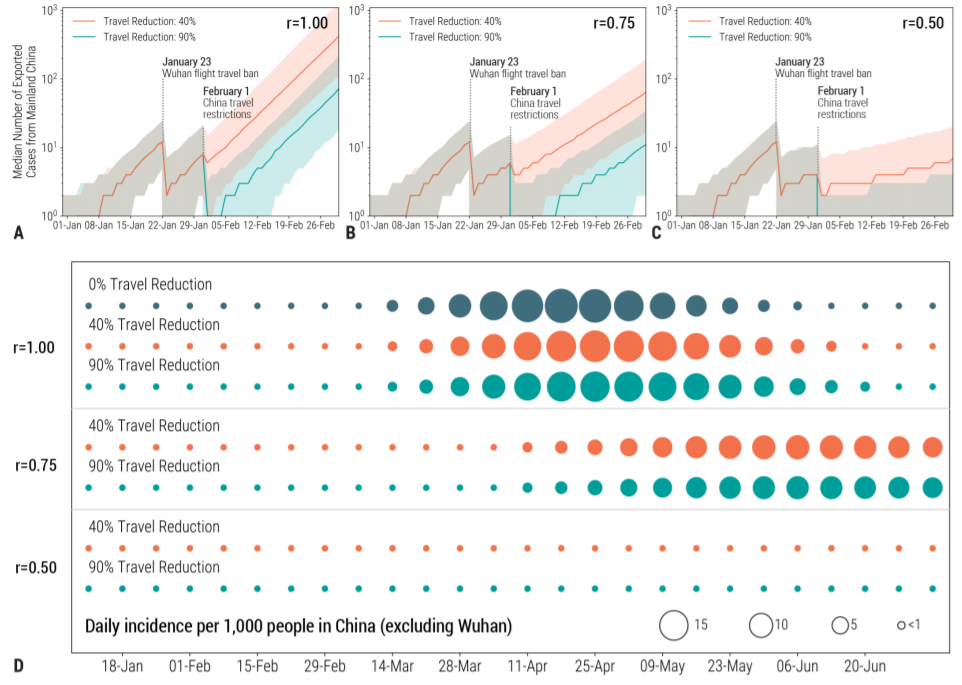
\includegraphics[width=.9\textwidth]{results_effect_travel_ban.png}
    \caption{Effets combinés des restrictions de voyage et de la réduction du taux de transmission sur l'épidémie. (A) Médiane du nombre total de cas importés de Chine continentale sans réduction de transmission ($r=1$), avec une réduction des déplacements de 40\% ou 90\%. (B) Comme (A) pour $r = 0.75$. (C) Comme (A) avec $r = 0.5$. Les zones d'ombres représentent les intervalles de confiance à 90\%. (D) Effets des différents scénarios sur la Chine continentale à l'exception de Wuhan.}
    \label{fig:results-effect-travel-ban}
\end{figure}

En revanche, si on réduit également le taux de transmission, les effets sont bien meilleurs. Dans le cas où $r=0.75$, l'évolution de la courbe ralentit, même si l'épidémie continue de progresser de façon notable (figures 1B et deuxième partie de 1D). Lorsque $r=0.5$, la progression de l'épidémie est largement réduite (figure 1C) et on ne distingue même plus de pic (troisième partie figure 1D). Cela illustre "l'aplatissement de la courbe" dont on entendait parler dans les médias il y a quelques semaines. De plus, cela justifie les campagnes de sensibilisation sur les gestes barrières ainsi que la politique de confinement, visant à forcer la "distanciation sociale", seule véritable moyen de réduire le taux de transmission.

\bibliographystyle{unsrt}
\bibliography{ref}
\end{document}